% appendix
\chapter{Filtering lists}
\label{sec:probe-filters}

\lstdefinelanguage{JavaScript}{
  keywords={break, case, catch, continue, debugger, default, delete, do, else, finally, for, function, if, in, const, instanceof, new, return, switch, this, throw, try, typeof, var, void, while, with},
  morecomment=[l]{//},
  morecomment=[s]{/*}{*/},
  morestring=[b]',
  morestring=[b]",
  sensitive=true
}



This appendix details the major technical filtering lists and annotations applied in Illumina 450K and EPIC methylation arrays to remove unreliable or ambiguous CpG probes. 

\subsection{Reducing the risk of false discovery enabling identification of biologically significant genome-wide methylation status using the humanmethylation450 array}
\label{app:naeem2014}



Naeem \emph{et al.} \cite{naeem2014} proposed a structured filtering framework to reduce false discoveries by sequentially discarding probes based on hybridisation specificity and genomic integrity (Figure \ref{fig:Workflow}).  
The main exclusion steps are:
\begin{enumerate}[label=-]
  \item Multi-mapping or cross-hybridising probes $\Rightarrow$ \textit{discard}.
  \item Probes overlapping repetitive elements (LINE/SINE/ALU) $\Rightarrow$ \textit{discard}.
  \item Probes targeting regions with INDELs $\Rightarrow$ \textit{discard}.
  \item Probes overlapping SNPs:
    \begin{enumerate}[label=--]
      \item SNP at CpG or extension site $\Rightarrow$ \textit{discard}.
      \item SNP near target but not interfering in bisulfite space $\Rightarrow$ \textit{keep}.
    \end{enumerate}
\end{enumerate}
The resulting ``discard'' set therefore removes probes affected by cross-reactivity, structural polymorphisms (INDELs), and SNPs that alter CpG interrogation.

\subsection{Discovery of cross-reactive probes and polymorphic cpgs in the illumina infinium humanmethylation450 microarray}
\label{app:chen2013}
Chen \emph{et al.} \cite{chen2013} empirically identified probes in the 450K array that exhibit off-target hybridisation or overlap with common SNPs.  
For this project, only the \textbf{cross-reactive list} is available and used.  
This list enumerates $\sim$29k multi-mapping probes whose methylation signal cannot be uniquely attributed to one genomic locus.

\subsection{Critical evaluation of the Illumina MethylationEPIC BeadChip microarray for whole-genome DNA methylation profiling}
\label{app:pidsley2016}
Pidsley \emph{et al.} \cite{pidsley2016} provide a platform-level assessment of the EPIC array, with explicit \emph{annotated probe lists} that flag probes whose methylation signal may be confounded by design- or genome-related artefacts. The focus is on probe categories and positions where technical bias arises, rather than on a universal, prescriptive blacklist. In particular, they catalogue:

\begin{itemize}[label=-]
  \item \textbf{Cross-hybridising CpG-targeting probes:} CpG probes showing sequence homology (off-target matches) to additional genomic loci, yielding non-unique hybridisation and potentially inflated or ambiguous $\beta$ signals.
  \item \textbf{Cross-hybridising non-CpG-targeting probes:} off-target issues among CNG/non-CpG probes; these are typically excluded in CpG-centric analyses due to limited interpretability and higher risk of artefacts.
  \item \textbf{Probes overlapping common genetic variation:} annotation of variants from population data at three critical positions:
  \begin{enumerate}[label=--]
    \item \textit{At the interrogated CpG} (polymorphic CpG) --- directly affects the presence of the CpG dinucleotide and the measured methylation state;
    \item \textit{At the single-base extension (SBE) site} (Type~I) --- perturbs extension and dye chemistry, biasing intensity ratios;
    \item \textit{Within the probe body} --- can reduce binding affinity or alter hybridisation kinetics, especially for common variants.
  \end{enumerate}
\end{itemize}


\subsection{Comprehensive characterization, annotation and innovative use of infinium dna methylation beadchip probes}
\label{app:zhou2016}
Zhou \emph{et al.} \cite{zhou2016} released a unified probe annotation for both 450K and EPIC arrays with multiple binary mask columns (\texttt{MASK\_*}).  
Each \href{https://zwdzwd.github.io/InfiniumAnnotation/mask.html}{mask} flags probes to be removed due to specific technical artifacts.
\begin{itemize}[label=-]
  \item \texttt{MASK.mapping}: probes with low or inconsistent mapping quality (non-unique alignment or presence of INDELs);
  \item \texttt{MASK.typeINextBaseSwitch}: Type-I probes carrying a SNP in the extension base that causes a color-channel switch (\emph{CCS} probes);
  \item \texttt{MASK.extBase}: probes whose extension base is inconsistent with the expected color channel or CpG context;
  \item \texttt{MASK.sub30.copy}: probes with non-unique 30-bp 3' subsequences (potential cross-hybridisation);
  \item \texttt{MASK.snp5.common}: probes overlapping a SNP within $\pm5$\,bp of the interrogated CpG (even with global MAF < 1\%);
  \item \texttt{MASK.snp5.GMAF1p}: probes overlapping SNPs with global MAF > 1\%;
  \item \texttt{MASK.general}: recommended composite mask integrating mapping, SNP, and cross-reactivity filters for general use;
  \item \texttt{MASK.rmsk15}: probes overlapping RepeatMasker regions (not recommended for exclusion in standard workflows).
\end{itemize}

This resource provides a programmatic and reproducible way to perform fine-grained probe masking.

\begin{figure}[t]
    \centering
    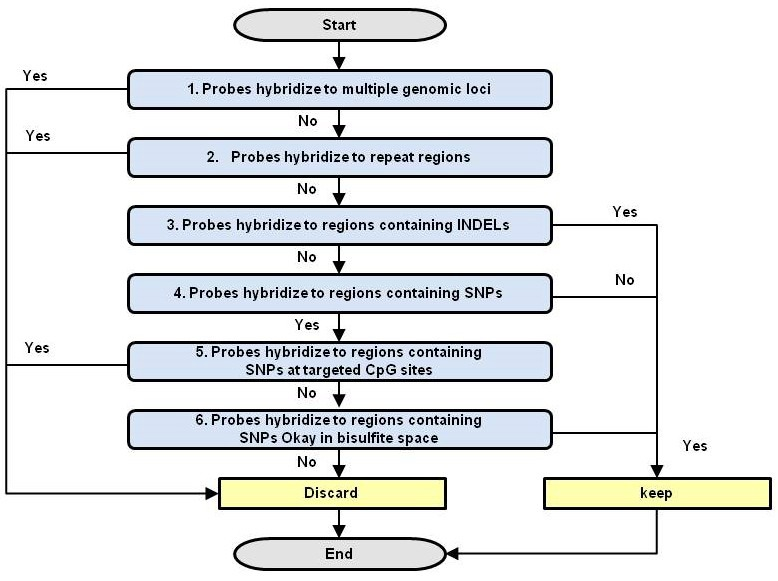
\includegraphics[width=0.4\textwidth]{images/appendix/Workflow for determining affected Probes.jpg}

     \caption{Workflow for determining affected Probes.}
    \label{fig:Workflow}
\end{figure}

\begin{table}[t]
\small
\caption{Technical categories covered by each filtering resource.}
\centerline{ % <-- USA QUESTO
\begin{tabular}{lccccc}
\toprule
\textbf{Category} & \textbf{Naeem} \ref{app:naeem2014} & \textbf{Chen} \ref{app:chen2013} & \textbf{Pidsley} \ref{app:pidsley2016} & \textbf{Zhou} \ref{app:zhou2016} & \textbf{McCartney} \ref{app:mccartney2016}\\
\midrule
Cross-hybridisation / multi-mapping & Yes (Steps 1–2) & Yes & Yes & \texttt{MASK\_mapping} & Table~2+3 \\
SNP at CpG / extension base   	& Yes (Step 5) & -- & Yes & \texttt{MASK\_snp5, MASK\_extBase} & -- \\
Nearby SNP tolerated   	& Conditional (Step 6) & -- & -- & -- & -- \\
INDEL / structural variant   	& Yes (Step 3) & -- & -- & -- & -- \\
Non-CpG probes   	& -- & -- & Yes 	& \texttt{MASK\_nonCG} & Table~3 \\

\bottomrule
\end{tabular}
} 
\end{table}

\subsection{Identification of polymorphic and off-target probe binding sites on the Illumina Infinium MethylationEPIC BeadChip}
\label{app:mccartney2016}
McCartney \emph{et al.} \cite{mccartney2016} assessed probe design artifacts and published supplementary tables that include:
\begin{itemize}[label=-]
  \item Cross-hybridising CpG-targeting probes;
  \item Cross-hybridising non-CpG-targeting probes.
\end{itemize}


